\documentclass[landscape, 11pt]{report}

% Packages
\usepackage[landscape]{geometry}
\usepackage{amsmath}
\usepackage{xcolor}
\usepackage[utf8]{inputenc}
\usepackage[russian]{babel}
\usepackage{geometry}
\usepackage{graphicx}

% Options
\graphicspath{ {../figures/} {./figures/}}
\geometry{left=2.5cm,right=2.5cm,top=2.5cm,bottom=2.5cm}
\setlength\parindent{0pt}

% Title
\title{
	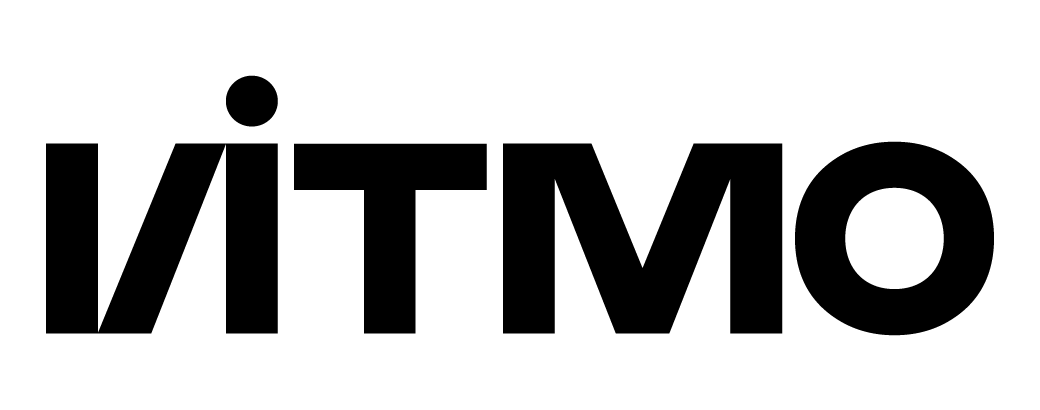
\includegraphics[scale=0.07]{logo}\\
	\vspace{0.5em}
	Языки программирования. Семантика и система типов\\
	\vspace{0.2em}
	\Large Теоретическое задание. Тема 10
}
\author{Бронников Егор}
\date{}


\begin{document}
	
	% Титул
	
	\maketitle
	
	\vspace{-0.5cm}
	\hrule
	\vspace{0.5cm}
	
	% Задание 1
	
	\textbf{Задание 1.} Реализуйте классы, соответствующие следующим императивным объектам на Welterweight Java. Можете использовать следующие определения \verb|Unit| и \verb|Nat|.
	
	\vspace{0.2cm}
	
	\verb|class Unit extends Object { }| \\
	\verb|class Nat extends Object { }| \\
	\verb|class Zero extends Nat { }| \\
	\verb|class Succ extends Nat { Nat n; }|
	
	\vspace{0.2cm}
	
	\textit{(a)} \verb|SetCounter|:
	
	\begin{verbatim}
		SetCounter =
		    { get : Unit -> Nat
		    , set : Nat -> Unit
		    , inc : Unit -> Unit
		    }
	\end{verbatim}
	
	\vspace{-0.1cm}
	
	\textit{(b)} \verb|InstrCounter| (реализация метода \verb|inc| не должна быть переопределена, вместо этого необходимо полагаться на открытую рекурсию):
	
	\begin{verbatim}
		InstrCounter =
		    { get : Unit -> Nat
		    , set : Nat -> Unit
		    , inc : Unit -> Unit
		    , accesses : Unit -> Nat
		    }
	\end{verbatim}
	
	\vspace{-0.1cm}

	\newpage

	\textit{Решение. Задание (а).}
	
	\vspace{-0.2cm}
	
	\begin{verbatim}
		class Unit extends Object { }
		class Nat extends Object { }
		class Zero extends Object { }
		
		class Succ extends Nat {
		    Nat n;
		
		    Succ(Nat n) {
		        this.n = n;
		    }
		}
	
		class SetCounter {
		    Nat value;
		
		    SetCounter() {
		        this.value = new Zero();
		    }
	    
		    Nat get(Unit u) {
		        return this.value;
		    }

		    Unit set(Nat n) {
		        this.value = n;
		        return new Unit();
		    }

		    Unit inc(Unit u) {
		        this.value = new Succ(this.value);
		        return new Unit();
		    }
		}
	\end{verbatim}
	
	\newpage

	\textit{Решение. Задание (b).}
	
	\vspace{-0.2cm}
	
	\begin{verbatim}
		class InstrCounter extends SetCounter {
		    SetCounter accessCount;
			
		    InstrCounter() {
		        super();
		        this.accessCount = new SetCounter();
		    }
			
		    Nat get(Unit u) {
		        accessCount.inc(u);
		        return super.get(u);
		    }
			
		    Unit set(Nat n) {
		        accessCount.inc(new Unit());
		        return super.set(n);
		    }
			
		    Unit inc(Unit u) {
		        accessCount.inc(u);
		        return super.inc(unit);
			}
		
		    Nat accesses(Unit u) {
		        return this.accessCount.get(u);
		    }
		}
	\end{verbatim}
	
	\vspace{0.2cm}
	\hrule
	
	\newpage

	% Задание 2
	
	\hrule
	\vspace{0.5cm}
	
	\textbf{Задание 2.} Для следующего примера программы на Welterweight Java, выпишите следующие моменты динамической семантики:
	
	\begin{itemize}
		\item[] (a) начальную конфигурацию;
		\item[] (b) последовательность правил динамической семантики (только названия правил в корректном порядке), которые будут применены при вычислении;
		\item[] (c) конечную конфигурацию.
	\end{itemize}
	
	\begin{center}
		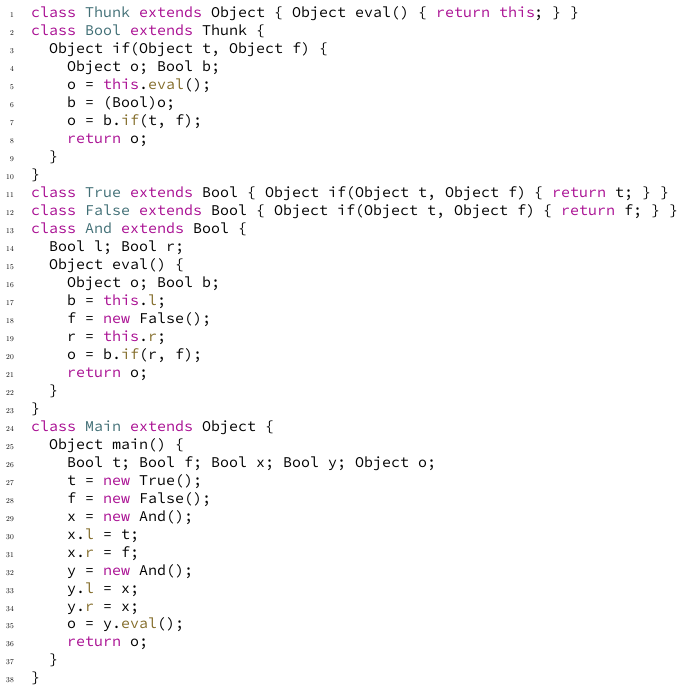
\includegraphics[scale=0.505]{code}
	\end{center}
	
	\newpage
	
	\textit{Решение.}
	
	\vspace{0.5cm}
	
	\textit{Задание (a).}
	
	\vspace{0.1cm}
	
	\textit{Ответ:} $H \; | \; <F, s> \; p_0$
	
	\vspace{0.5cm}
	
	\textit{Задание (b).}
	
	\vspace{0.1cm}
	
	\textit{Ответ:}
	
	\begin{center}
		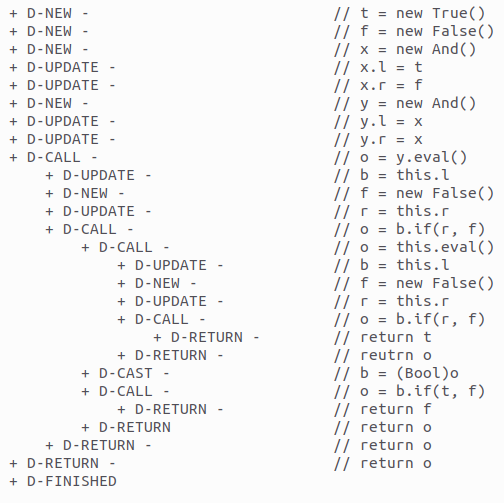
\includegraphics[scale=0.6]{solution}
	\end{center}

	\vspace{0.5cm}

	\textit{Задание (c).}
	
	\vspace{0.1cm}
	
	\textit{Ответ:} $False$	
	
	\vspace{0.2cm}
	\hrule
	
\end{document}
